We conducted several numerical experiments to confirm the validity of the error bounds formed in \cref{sec:mpanalysis} by varying size for all algorithms, block sizes in {\tt mpBQR3}, and comparing {\tt mpHQR2} against {\tt mpTSQR2} with varying condition numbers.
We used Julia, a programming language which allows fp16 storage and {\tt castup} and {\tt castdown} operations between types in {fp16, fp32, fp64}, but no built-in fp16 arithmetic.
Therefore, we relied on using \cref{algo:simulate} for $f\in \text{OP} \cup\{{\tt dot\_product}\}$ to simulate \cref{assump:mp} and TensorCore bFMAs.\par

In \cref{sec:algo,sec:mpanalysis}, we gave the forward error bounds for $\bb{R}$ and $\bb{Q}$ separately. 
Since our numerical experiments instead measure a backward error, $\|\hat{\bb{Q}}\hat{\bb{R}}-\bb{A}\|_F$, and an orthogonal error, $\|\hat{\bb{Q}}^{\top}\hat{\bb{Q}}-\bb{I}\|_2$, we show how to convert general forward errors into those computed quantities.
Given $\|(\hat{\bb{R}}-\bb{R})[:,j]\|_2\leq \epsilon_R \|\bb{A}[:,j]\|_2$ and $\|\hat{\bb{Q}}-\bb{Q}\|_F\leq \epsilon_Q$,
\begin{align}
	\|(\hat{\bb{Q}}\hat{\bb{R}}-\bb{A})[:,j]\|_2 &\leq (\epsilon_R+\epsilon_Q + \epsilon_R\epsilon_Q)\|\bb{A}[:,j]\|_2,\;\; j=1:n,\quad \text{see \cite{Higham2002}},\\
	\|\hat{\bb{Q}}\hat{\bb{R}}-\bb{A}\|_F &\leq n^{1/2}(\epsilon_R+\epsilon_Q + \epsilon_R\epsilon_Q)\|\bb{A}\|_F, \label{eqn:QRA} \\
	\|\hat{\bb{Q}}^{\top}\hat{\bb{Q}}-\bb{I}\|_2 &\leq \|\hat{\bb{Q}}^{\top}\hat{\bb{Q}}-\bb{I}\|_F \simeq 2\epsilon_Q,\quad\text{see \cite{Mori2012}} \label{eqn:QQI}.
\end{align}
First, we tested \cref{algo:hhQR,algo:blockHQR,algo:par_tsqr,algo:mpBQR}, {\tt mpHQR2}, {\tt mpBQR2}, and {\tt mpTSQR2} for varying matrix sizes.
%Then, we compared the performance of {\tt mpHQR2} and {\tt mpTSQR2}, and lastly, tested varying block sizes in \cref{algo:mpBQR} for a fixed matrix size. 
%The left plot of \cref{fig:sizemp3} shows the backward error for HQR, BQR, TSQR, and their mixed precision variants.
We increased the number of rows $m$ from $1000$ to $13949$, 
% $18694$
while keeping $n=m/4$, $r=n/4$, and $L=2$ and the test matrices were sampled from the standard normal distribution. 
On the left plot of \cref{fig:sizemp3}, we see three clusters which each correspond to: top, \cref{assump:mp}; middle, TensorCore bFMAs; and bottom, uniform precision implementations in fp32.
The high precision and bFMA implementations scale similarly to each other when increasing the matrix size, whereas the \cref{assump:mp} variants grow unstable more quickly.
In addition, while HQR, BQR, and TSQR perform similarly in high precision and when using bFMAs, {\tt mpTSQR2} is less accurate by a quarter to a half order of magnitude in comparison to {\tt mpBQR2} and {\tt mpHQR2}.
The specifications for $m,n,L,M_{l,h}$ for this experiment derive the upper bound for $\|\Delta \bb{Q}_{mpTSQR2}\|_F$, \cref{eqn:mptsqr2Q}, to be larger than that of $\|\Delta \bb{Q}_{mpHQR2}\|_F$, \cref{eqn:mpHQR2Q}.
However, a more careful comparison of {\tt mpHQR2} and {\tt mpTSQR2} show that there exists a regime where {\tt mpTSQR2} can outperform {\tt mpHQR2}.
\begin{figure}[h!]%{r}{.53\textwidth}
	\centering
	\vspace{-10pt}
	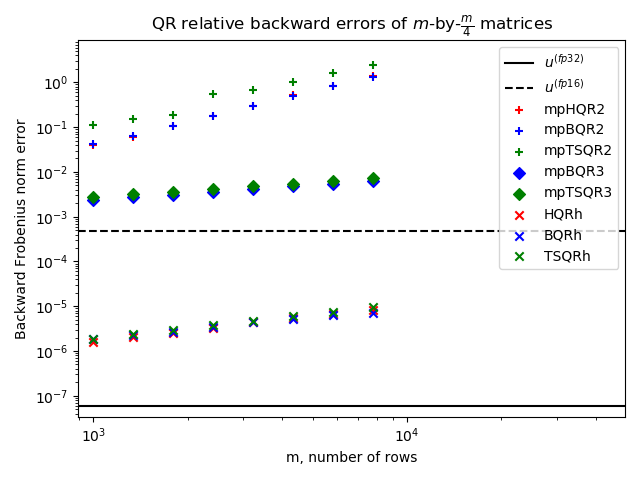
\includegraphics[width=0.45\textwidth]{./figures/sizefig.png}
	%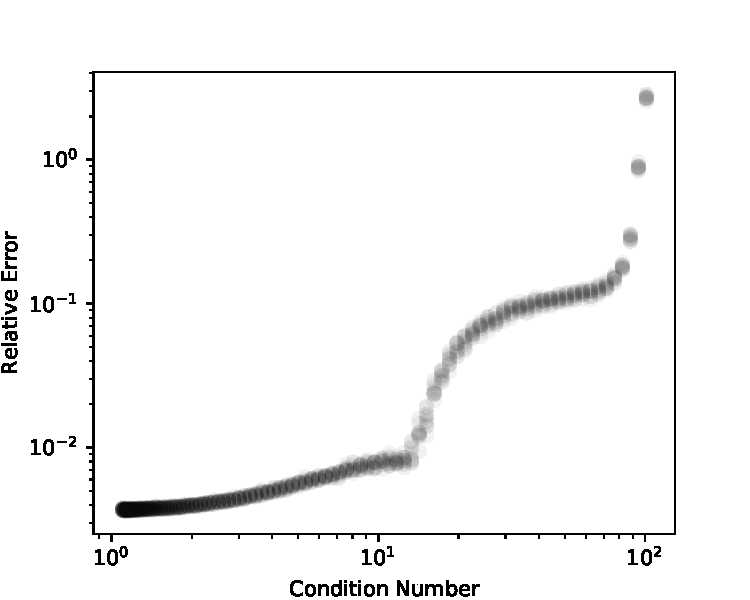
\includegraphics[width=0.45\textwidth]{./figures/unblocked.pdf}
	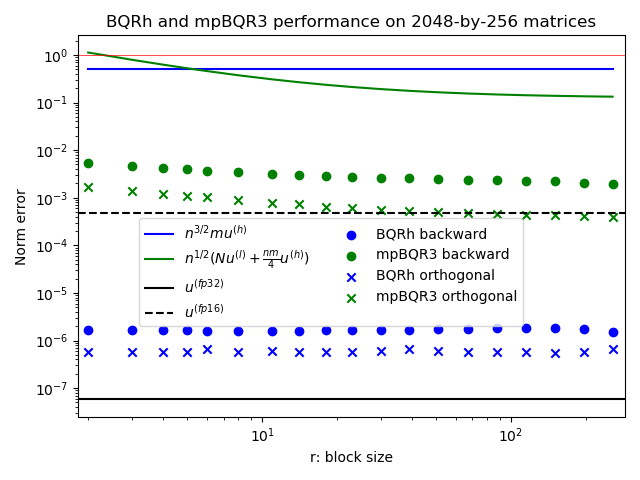
\includegraphics[width=0.45\textwidth]{./figures/mpBQR3-blocksize-1108.png}
	\caption{\label{fig:sizemp3}Left plot: Backward errors of HH QR factorization algorithms in \cref{sec:algo,sec:mpanalysis} with varying matrix sizes. 
		%Right plot: {\tt mpHQR2} errors for $4000$-by-$100$ matrices with varying condition numbers.}
		Right plot: Norm errors of fp32 BQR and {\tt mpBQR3} for $2048$-by-$256$ matrices for varying block sizes.}
	\vspace{-10pt}
\end{figure} 

Next, we varied the block sizes for performing fp32 BQR and {\tt mpBQR3} on $2048$-by-$256$ sized matrices, which were chosen to yield error bounds below 1 for both algorithms.
The right plot of \cref{fig:sizemp3} shows the error bounds and the computed value for the backward error for the two algorithms where the block size $r$ varies from $2$ to $256$. 
The test matrices were generated following example from \cite{Blanchard2019} by setting $\bb{A}={\tt castdown}(\bb{Q}_1\bb{D}\bb{Q}_2)$ where $\bb{Q}_1\in\F_h^{m\times n}$, $\bb{Q}_2\in\F_h^{n\times n}$ are orthogonal and $\bb{D}=\mathrm{Diagonal}(\{\log_{10}(0),\cdots, \log_{10}(-3)\})\in\F_h^{n\times n}$.  
The high precision implementation yields backward error close to $u^{(fp32)}$ and {\tt mpBQR3} yields errors near $u^{(fp16)}$ that follows the downward trend suggested by \cref{eqn:mpBQR3}.
As block sizes increase, {\tt mpBQR3} grows more accurate. 
This trend correlates to $1/N$, the approximate fraction of FLOPs in {\tt mpBQR3} performed in high precision, marked in orange.
%TODO: line Q.
However, the rightmost data for {\tt mpBQR3} (corresponds to $r=n$), is still between 3 and 4 orders of magnitude less accurate than its high precision variant. 
Further studies that directly test speed-ups from bFMAs against the accuracy of {\tt mpBQR3} are needed to fully understand the potential uses for mixed precision QR algorithms.
%There exist applications that are robust to QR factorization errors and could benefit from speed-ups of using bFMAs.

Lastly, we compared {\tt mpTSQR2} against {\tt mpHQR2}.
Note that an empirical comparison of the two algorithms implemented in fp64 arithmetic were reported in \cite{Mori2012}, and we omit the comparison against {\tt mpBQR2} since it performs very similarly to {\tt mpHQR2}.
Following example from \cite{Mori2012}, we used $m$-by-$n$ random matrices, $\bb{A}_{\alpha} = \bb{Q'}(\alpha \bb{E} + \bb{I})/\|\bb{Q'}(\alpha \bb{E} + \bb{I})\|_F$, where $\bb{Q'}\in\mathbb{R}^{m\times n}$ is orthogonal and $\bb{E}\in\R^{n\times n}$ is the matrix of $1$'s. 
We constructed $\bb{Q'}$ by computing the default QR factorization of matrix $\bb{\Omega}\in\F_{fp64}^{4000\times100}$ in Julia, which performs BQR with $r=36$ entirely in fp64 arithmetic, and elements of the random matrix $\bb{\Omega}$ were sampled from the uniform distribution over $[0,1]$.
By construction, $\bb{A}_{\alpha}$ has 2-norm condition number $n\alpha+1$. 
By varying $\alpha$ from {\tt 1e-4} to {\tt 1}, we varied the condition number from $1.1$ to $101$, and we generated $10$ samples for each value of $\alpha$.
The relative backward error, $\|\hat{\bb{Q}}\hat{\bb{R}}-\bb{A}\|_F/\|\bb{A}\|_F$, was computed by casting up $\hat{\bb{Q}}$, $\hat{\bb{R}}$, and $\bb{A}$ to fp64 to compute the Frobenius norms.
Plugging in $m=4000$, $n=100$, $u^{(l)}=u^{(fp16)}$, $u^{(h)}=u^{(fp32)}$, and $c=1$ (for $\tilde{\gamma}$) into the error bounds for {\tt mpHQR2} combined with \cref{eqn:QRA,eqn:QQI} are approximately {\tt 1.179} and {\tt 1.146}.
These error bounds are \emph{relative} and these worst-case bounds do not guarantee errors below 100\%.
The TSQR bounds for the same parameters for $L=1:5$ are even larger, which indicates that stability is not guaranteed. 
The leftmost plot of \cref{fig:allTSQR} shows the backward errors of {\tt mpHQR2} increasing as the theoretical condition numbers of the generated random matrices increase, and these errors correspond to the error data on the vertical axis, $L=0$, of the middle plot.
In addition to the errors from {\tt mpHQR2}, Figure~\ref{fig:allTSQR} shows the errors from {\tt mpTSQR2s} of levels varying from $L=1$ to $L=5$, where each line represents the errors of HQR and variants of TSQR calculated from the same random test matrix.
Figure~\ref{fig:allTSQR} reveals two different trends for the errors as we deepen the complexity of the QR algorithm from {\tt mpHQR2} to {\tt mpTSQR2} with $L=5$. 
One trend occurs for matrices with smaller condition numbers, where {\tt mpHQR2} is stable, but {\tt mpTSQR2} with higher levels yield larger errors. 
Another trend occurs for matrices with higher condition numbers, where single-level and 2-level {\tt mpTSQR2} yield smaller errors than {\tt mpHQR2}. 
In these cases, errors from {\tt mpTSQR2} with 3 or more levels are similar to or worse than their 2-level variants, but generally do not exceed those of {\tt mpHQR2} most of the times.
These results suggests that TSQR can outperform HQR even in mixed precision settings, and particularly when HQR is unstable due to larger condition numbers.
%Although this experiment focused on condition numbers, identifying other properties that point to better performance of TSQR than HQR can further broaden the potential use of mixed precision TSQR in applications.
\begin{figure}[h!]%{r}{.53\textwidth}
	\centering
	%\vspace{-10pt}
	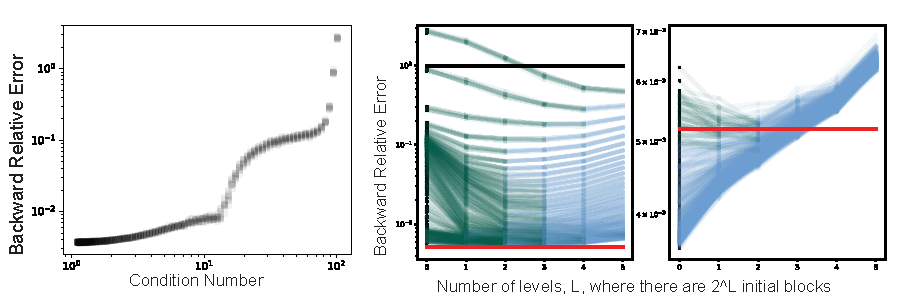
\includegraphics[width=\textwidth]{./figures/allTSQR3.pdf}
	%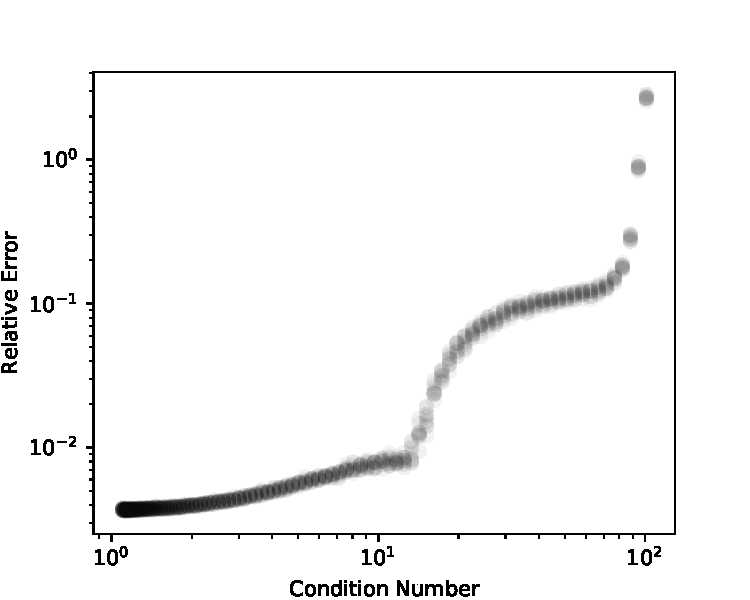
\includegraphics[width=0.35\textwidth]{./figures/unblocked.pdf}
	%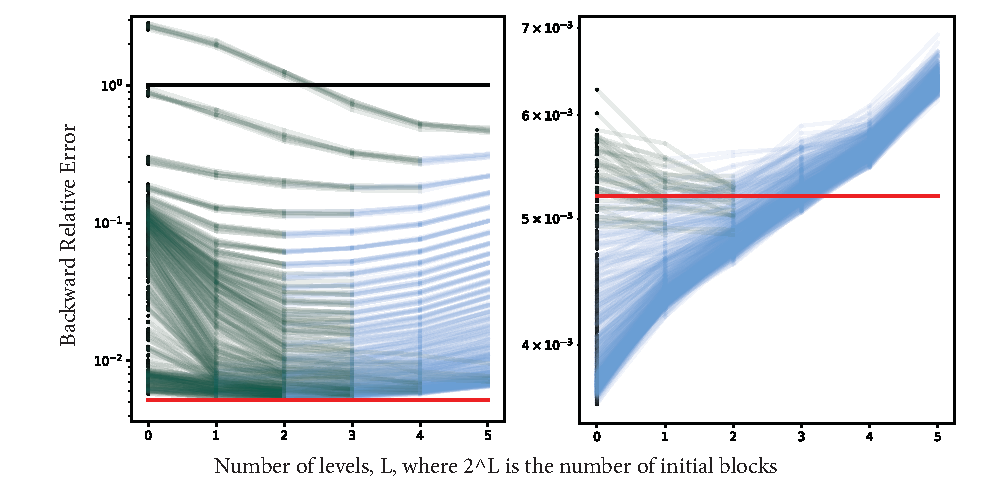
\includegraphics[width=0.64\textwidth]{./figures/allTSQR2.pdf}
	\vspace{-15pt}
	\caption{\label{fig:allTSQR} All plots show the backward relative error for 4000-by-100 sized test matrices. Left: {\tt mpHQR2} on condition numbers ranging from 1.1 to 101;  Middle: {\tt mpTSQR2} on condition numbers ranging from 5.3 to 101; Right:  {\tt mpTSQR2} on condition numbers ranging from 1.1 to 5.3. }
	\vspace{-15pt}
\end{figure}

In conclusion, most of the experiments display the trends that error bounds in \cref{sec:algo,sec:mpanalysis} suggest, and bFMA variants perform in between the high precision and \cref{assump:mp} variants as expected.
Also, a special case is shown that demonstrate {\tt mpTSQR2} can outperform {\tt mpHQR2} despite having higher error bounds.
All of the experiments showed that the actual errors were many orders of magnitude lower than the error bounds even when ill-conditioned, but this discrepancy varied for different mixed precision settings.
For example, backward and forward errors of {\tt mpBQR3} were \emph{only} 2-3 orders of magnitude below the error bounds, whereas the fp32 implementation of BQR yielded errors up to 6 orders of magnitude below the error bounds.
Although further studies with larger problem sizes and timings would be beneficial in developing an {\tt mpBQR3} with the optimal block size, $r$, our experiments confirm the intuition built from the error analysis in \cref{sec:mpanalysis}.